\begin{figure}[htb]
	\centering
	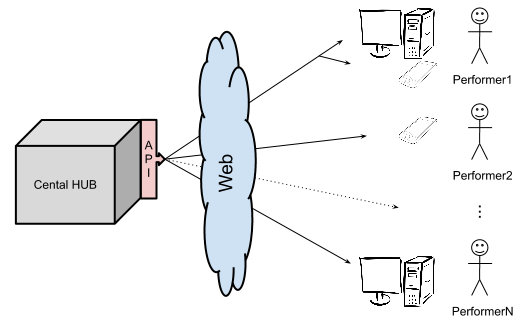
\includegraphics[width=0.75\columnwidth]{Architecture}
	\caption{Reference architecture.}
	\label{fig:architecture}
\end{figure}
% TODO nell'immagine metto anche un dispositivo mobile e un utente con 2 device

During the Design Process we faced the problem of finding a suitable Architectural
Model able to support all the requirements, in terms of flexibility and pluggability,
raised during the Process Design. In our model we use as a reference architecture
the one depicted in \autoref{fig:architecture}. Here we have a central hub
in charge of distributing the Tasks to the nodes\footnote{We refer to nodes
because we want to enclose both humans and devices.} and an abstraction layer.

The \emph{Central Hub} is used to manage all the data exchange between to the
nodes and the hub itself, orchestrating all the communication flow.

The \emph{Abstraction Layer} is used to normalize the differences between the
nodes, creating a coherent representation of nodes.\\




As described in \ref{design:work}, our framework has multiple configuration
points used to customize the Task behavior. As described in \vref{data:task},
for each Task we identified seven configuration points:
\begin{description}
	\item[\utask{} planning strategy:] defines how many \utask{} to create for
	each Task and associate the right portion of Objects to each of them.
	\item[\utask{} implementation strategy:] defines the logic behind the choice
	of a \utask{} implementation sent to a user.
	\item[Performer assignment strategy:] in charge of choosing the users who
	are suitable to execute a certain Task.
	\item[Task Planning strategy:] orchestrates the invocation of the \utask{}
	planning strategy, the \utask{} implementation strategy and the Performer
	assignment strategy.
	\item[Task Control strategy:] defines a controller for the Task, able to
	check the status, and if needed, perform corrective actions.
	\item[Aggregation function:] is in charge of joining the results obtained
	from the \utask{}s execution and create a Task output.
	\item[Emission policy:] is used to rule notifications sent to the Subscribers.
\end{description}
All these configuration points are described in \ref{sec:model:strategies}.